\documentclass[a4paper,14pt]{extarticle}

\usepackage[left=30mm, right=10mm, top=20mm, bottom=20mm]{geometry}

\usepackage{amssymb}
\usepackage{amsmath}
\usepackage{tikz}
\usepackage{pgfplots}

\usepackage{graphicx}
\usepackage{setspace}

\usepackage{minted}
\usepackage{xcolor}

\usepackage{siunitx}
\usepackage{booktabs}

\usepackage[T2A]{fontenc}
\usepackage[utf8]{inputenc}
\usepackage[russian]{babel}
\usepackage{tempora}
\usepackage{type1cm}
\usepackage{indentfirst}

\usepackage{caption}
\usepackage{subcaption}
\usepackage[hidelinks]{hyperref}
\usepackage[russian]{cleveref}
\usepackage{bookmark}

\onehalfspacing

\renewcommand{\theFancyVerbLine}{%
	\sffamily\small\color{black}\arabic{FancyVerbLine}%
}

\definecolor{codebg}{rgb}{0.12,0.12,0.14}
\definecolor{codeframe}{rgb}{0.40,0.40,0.45}
\definecolor{keywordcolor}{rgb}{0.45,0.65,1.0}
\definecolor{stringcolor}{rgb}{1.0,0.55,0.45}
\definecolor{commentcolor}{rgb}{0.55,0.75,0.60}
\definecolor{textcolor}{rgb}{0.90,0.90,0.90}

\setminted{
    bgcolor=codebg,
	fillcolor=codebg,
	framesep=1em,
	frame=single,
    rulecolor=\color{codeframe},
    fontsize=\normalsize,
    baselinestretch=1.1,
    linenos,
    numbersep=6pt,
    tabsize=4,
    breaklines,
    breakbytoken,
	breaksymbolleft={},
    autogobble,
    showspaces=false,
    showtabs=false,
}

\usemintedstyle{lightbulb}
\setmintedinline{
    bgcolor=codebg
}

\makeatletter
\setlength{\@fptop}{0pt}
\setlength{\@fpsep}{8pt}
\setlength{\@fpbot}{0pt plus 1fil}
\makeatother

\begin{document}
    \begin{titlepage}
		\centering
		
		
\includegraphics{images/FEFU-logo.jpg}\\
		МИНИСТЕРСТВО ОБРАЗОВАНИЯ И НАУКИ РОССИЙСКОЙ ФЕДЕРАЦИИ\\
		Федеральное государственное автономное образовательное учреждение высшего образования\\
		\textbf{«Дальневосточный федеральный университет»}

		\rule{\linewidth}{0.8mm}\\[0.3cm]
		
		\textbf{ИНСТИТУТ МАТЕМАТИКИ И КОМПЬЮТЕРНЫХ ТЕХНОЛОГИЙ}\\
		\textbf{Кафедра математического и компьютерного моделирования}\\
		\vspace*{0.9cm}
		
		Кулахсзян Сергей Грайрович\\
        \vspace*{0.3cm}

		ЭМПИРИЧЕСКАЯ ФУНКЦИЯ РАСПРЕДЕЛЕНИЯ \\
		\vspace*{0.3cm}

		\textbf{ЛАБОРАТОРНАЯ РАБОТА № 3}\\
		\vspace*{0.3cm}
		
		Направление подготовки 02.03.01сцт Сквозные цифровые технологии,\\ 
        бакалавриатская программа «Математика и компьютерные науки»\\ 
        Очной формы обучения\\
		\vspace{1.5cm}

		
		\vfill
		\centering
		г. Владивосток\\
		2026
	\end{titlepage}

    \tableofcontents
	\newpage

    \section{Построение эмпирической функции распределения с доверительным интервалом}

    Эмпирической функцией распределения является функция вида: \\
    $\displaystyle F^*(x) = \frac{m_x}{n}$, \\
    где $m_x$ -- число вариант выборки меньше или равно $x$, $n$ -- объём выборки.

    Доверительным интервалом функции распределения является вероятность неравенства: \\
    $\displaystyle
    P(U(x) < F^*(x) < L(x)) \geq 1 - \alpha, \\
    $
    где $1 - \alpha$ -- уровень доверия, $(U(x), L(x))$ -- доверительный интервал, вычисляемый по формуле: \\
    $\displaystyle
    L(x) = \max(F^*(x) - \varepsilon; 0) \\
    U(x) = \min(F^*(x) + \varepsilon; 1) \\
    \varepsilon = \sqrt{\displaystyle \frac{1}{2n} \ln \left(\frac{2}{\alpha} \right)}
    $

    Таким образом код для него вышел таким:
    \begin{minted}{python3}
def empiric_distribution_function(data: np.ndarray, x: float, alpha: float = 0.05) -> tuple[int, tuple[float, float]]:
    data = np.sort(data)
    n = len(data)
    
    value = np.where(data <= x)[0].size / n

    epsilon = np.sqrt(np.log(2 / alpha) / (2 * n))
    
    lower_bound = max(0, value - epsilon)
    upper_bound = min(1, value + epsilon)
    
    return value, (lower_bound, upper_bound)
    \end{minted}

    \section{Сравнение истинной функции распределения и эмпирической функций распределения}

    Код:
    \begin{minted}{python3}
def plot_all_distribution_functions(data: dict[str, dict[int, dict]]) -> None:
    fig, axes = plt.subplots(4, 2, figsize=(17, 22))
    fig.subplots_adjust(hspace=0.4, wspace=0.3)
    
    distribution_names = ["uniform", "bernoulli", "binom", "norm"]
    sizes = [100, 1000]
    
    for i, distribution in enumerate(distribution_names):
        for j, size in enumerate(sizes):
            ax = axes[i, j]
            sample = data[distribution][size]["X"]
            sample_sorted = np.sort(sample)
            
            x_min, x_max = sample_sorted[0], sample_sorted[-1]
            x_range = np.linspace(x_min, x_max, size)
            
            if distribution == "uniform":
                true_cdf = stats.uniform.cdf(x_range, loc=-1, scale=5)
            elif distribution == "bernoulli":
                true_cdf = stats.bernoulli.cdf(x_range, p=0.25)
            elif distribution == "binom":
                true_cdf = stats.binom.cdf(x_range, p=0.25, n=17)
            elif distribution == "norm":
                true_cdf = stats.norm.cdf(x_range, loc=15, scale=5)
            
            l1, = ax.plot(x_range, true_cdf, color='blue', label='Истинная функция распределения', linewidth=2)
            
            values = []
            lower_bounds = []
            upper_bounds = []
            
            for x in x_range:
                val, (low, upp) = empiric_distribution_function(sample, x)
                values.append(val)
                lower_bounds.append(low)
                upper_bounds.append(upp)
            
            l2, = ax.step(x_range, values, color='red', label='Эмпирическая функция распределения', where='post')
            
            l3, =ax.step(x_range, lower_bounds, color='green', linestyle='--', label='Доверительный интервал 95%', alpha=0.8, where='post')
            ax.step(x_range, upper_bounds, color='green', linestyle='--', alpha=0.8, where='post')
            
            ax.set_title(f"{distribution.capitalize()} (n={size})")
            ax.set_ylim(-0.05, 1.05)
            ax.grid(True, alpha=0.3)
            if i == 0 and j == 0:
                lines = [l1, l2, l3]
                labels = [l.get_label() for l in lines]

    fig.subplots_adjust(hspace=0.4, wspace=0.3, top=0.94)
    fig.legend(lines, labels, loc='upper center', ncol=1, frameon=True, bbox_to_anchor=(0.5, 0.98))
    plt.show()

plot_all_distribution_functions(data)
    \end{minted}

    Результат графиков:
    \begin{figure}[ht!]
        \centering
        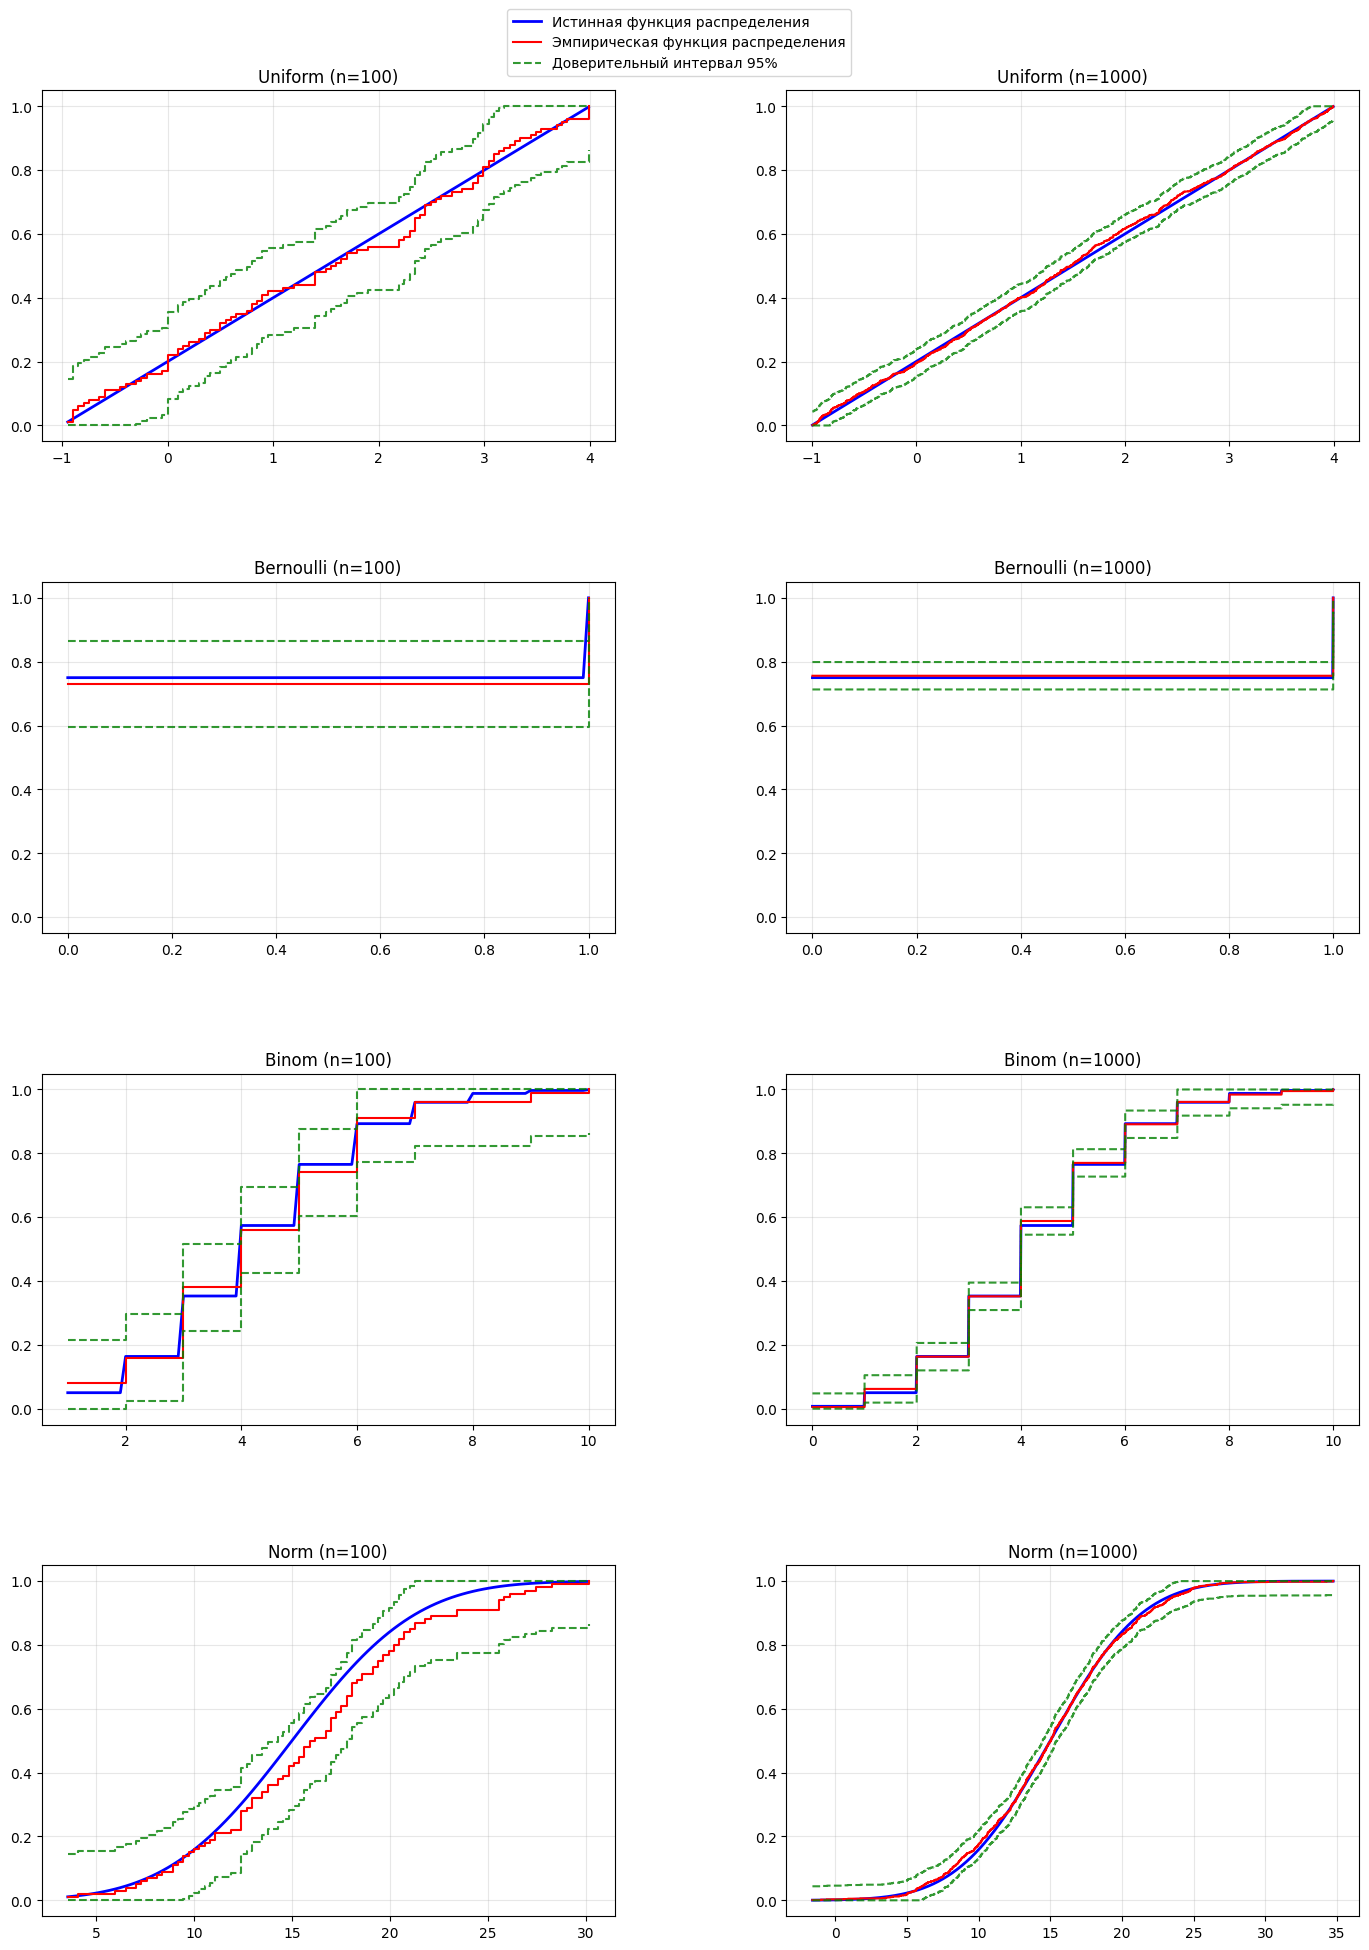
\includegraphics[width=0.99\textwidth]{images/distribution_graphics.png}
    \end{figure}

    \section{Сравнение истинной функции распределения и эмпирической функции распределения из scipy}

    Код:
    \begin{minted}{python3}
def plot_all_distribution_functions_scipy(data: dict[str, dict[int, dict]]) -> None:
    fig, axes = plt.subplots(4, 2, figsize=(17, 22))
    fig.subplots_adjust(hspace=0.4, wspace=0.3)
    
    distribution_names = ["uniform", "bernoulli", "binom", "norm"]
    sizes = [100, 1000]
    
    for i, distribution in enumerate(distribution_names):
        for j, size in enumerate(sizes):
            ax = axes[i, j]
            sample = data[distribution][size]["X"]
            sample_sorted = np.sort(sample)
            
            x_min, x_max = sample_sorted[0], sample_sorted[-1]
            x_range = np.linspace(x_min, x_max, size)
            
            if distribution == "uniform":
                true_cdf = stats.uniform.cdf(x_range, loc=-1, scale=5)
            elif distribution == "bernoulli":
                true_cdf = stats.bernoulli.cdf(x_range, p=0.25)
            elif distribution == "binom":
                true_cdf = stats.binom.cdf(x_range, p=0.25, n=17)
            elif distribution == "norm":
                true_cdf = stats.norm.cdf(x_range, loc=15, scale=5)
            
            l1, = ax.plot(x_range, true_cdf, color='blue', label='Истинная функция распределения', linewidth=2)
            
            ecdf_result = stats.ecdf(sample)
            values = ecdf_result.cdf.evaluate(x_range)
            continued_interval = ecdf_result.cdf.confidence_interval(confidence_level=0.95)
            
            l2, = ax.step(x_range, values, color='red', label='Эмпирическая функция распределения scipy.stats', where='post')
            
            l3, = ax.step(x_range, continued_interval.low.evaluate(x_range), color='green', linestyle='--', label='Доверительный интервал 95% scipy.stats', alpha=0.8, where='post')
            ax.step(x_range, continued_interval.high.evaluate(x_range), color='green', linestyle='--', alpha=0.8, where='post')
            
            ax.set_title(f"{distribution.capitalize()} (n={size})")
            ax.set_ylim(-0.05, 1.05)
            ax.grid(True, alpha=0.3)
            if i == 0 and j == 0:
                lines = [l1, l2, l3]
                labels = [l.get_label() for l in lines]

    fig.subplots_adjust(hspace=0.4, wspace=0.3, top=0.94)
    fig.legend(lines, labels, loc='upper center', ncol=1, frameon=True, bbox_to_anchor=(0.5, 0.98))
    plt.show()

plot_all_distribution_functions_scipy(data)
    \end{minted}

    Результат графиков:
    \begin{figure}[ht!]
        \centering
        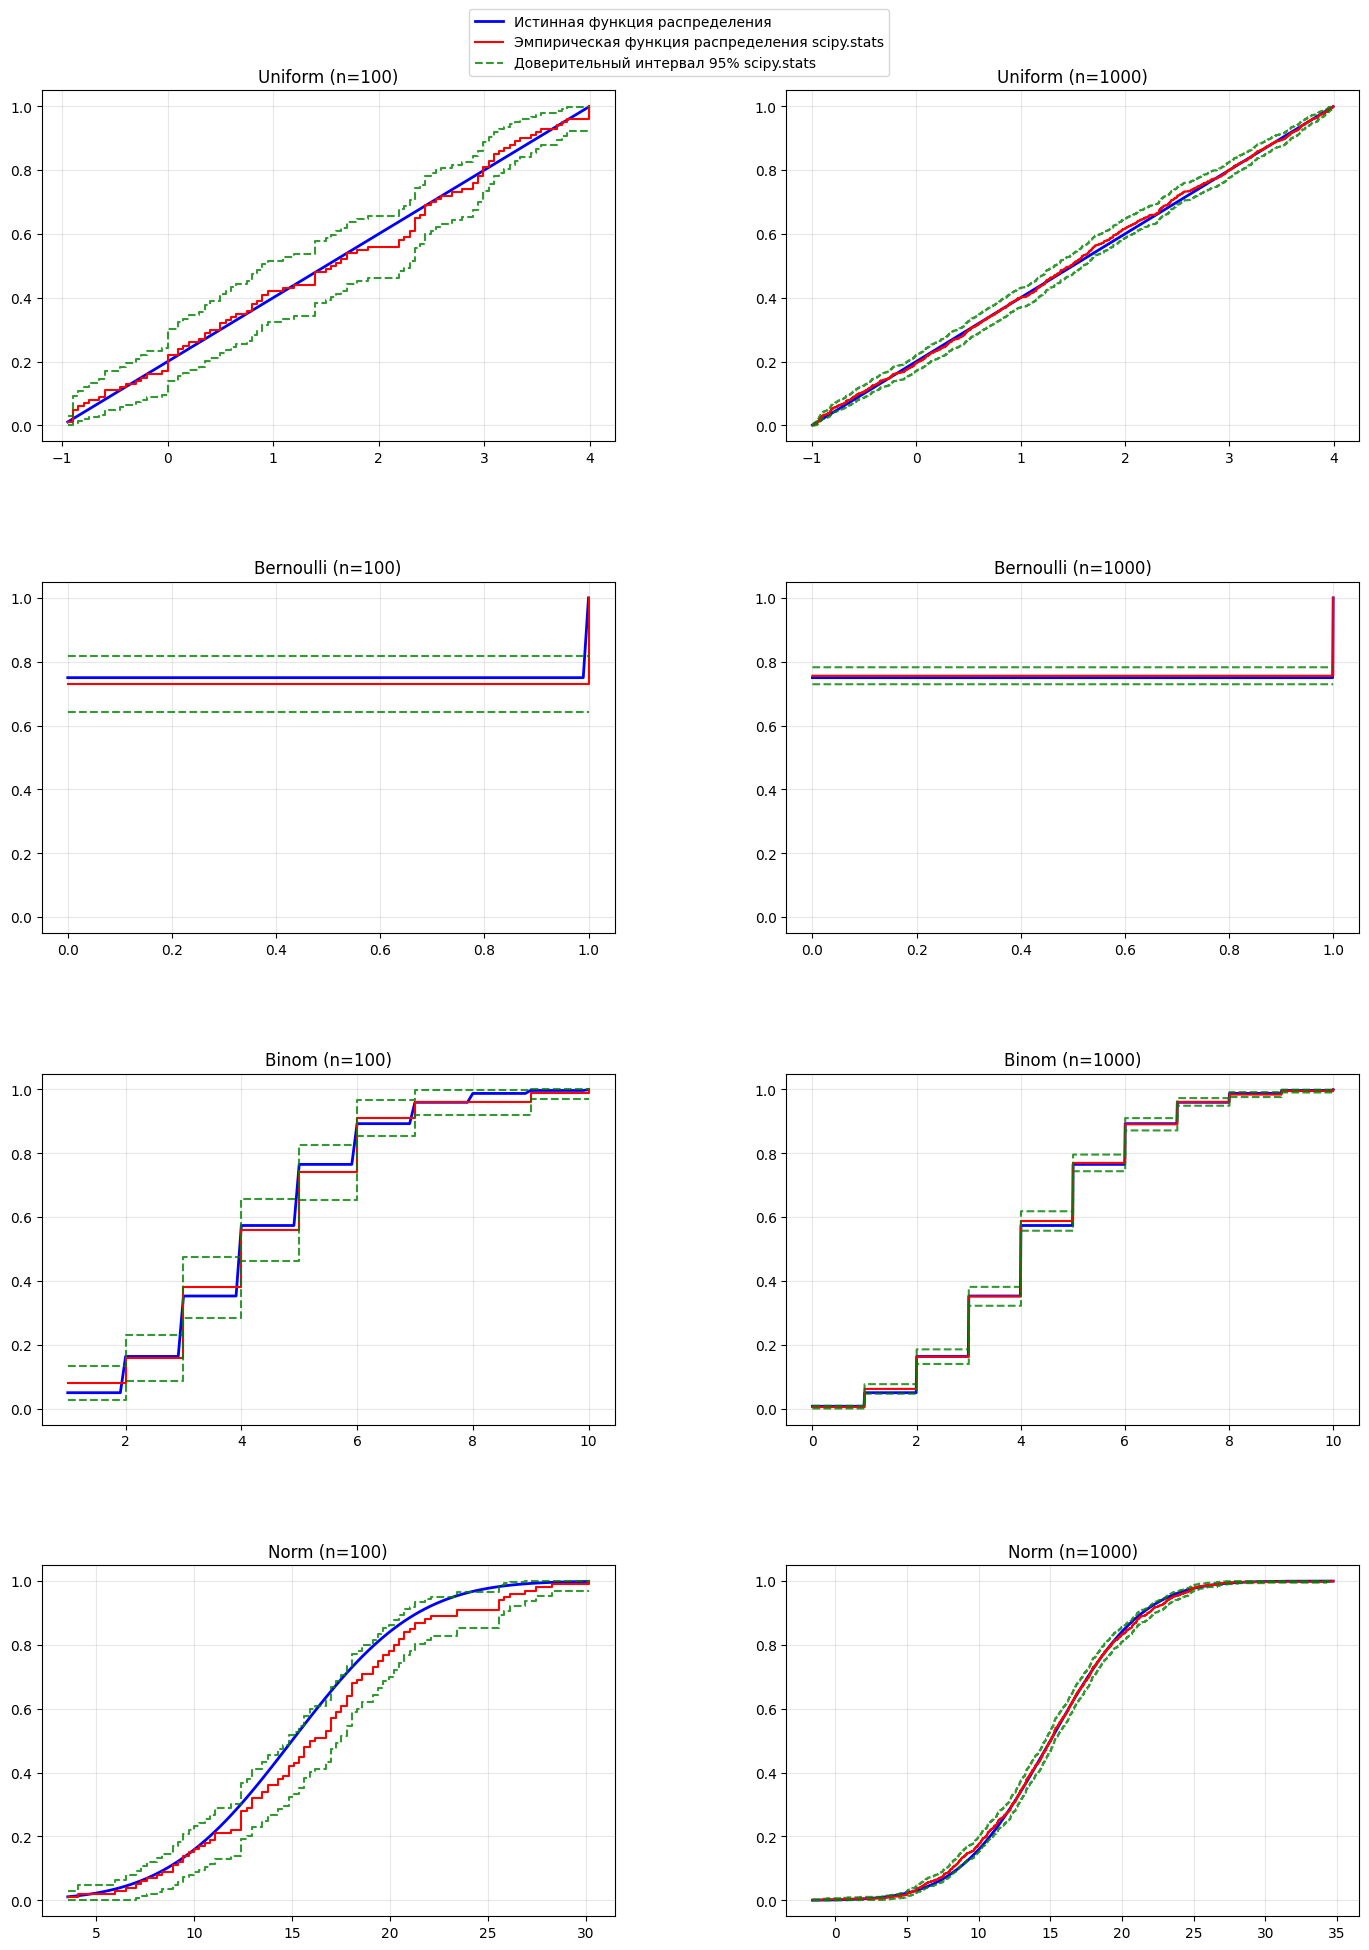
\includegraphics[width=0.99\textwidth]{images/distribution_graphics_scipy.png}
    \end{figure}

\end{document}
